%buck
\documentclass[tikz,border=2pt]{standalone}
\usepackage[american]{circuitikz}
\begin{document}

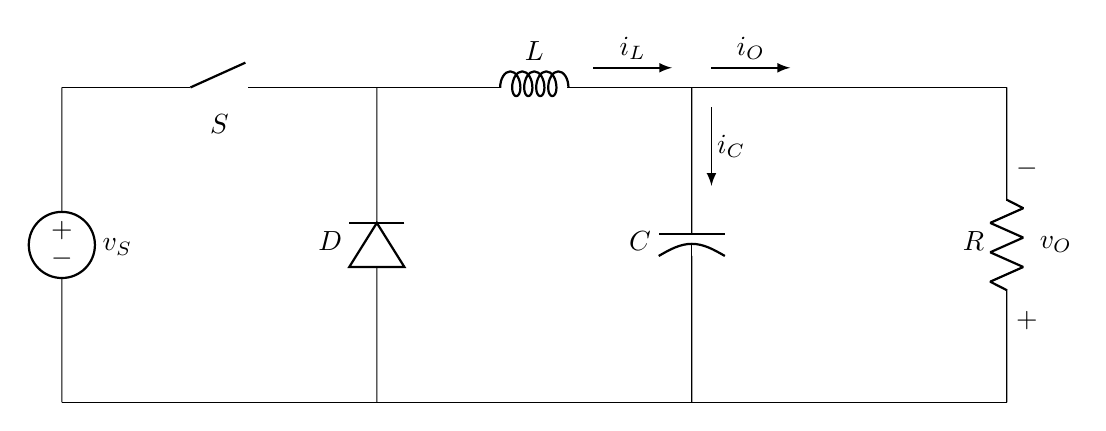
\begin{tikzpicture}[transform shape, american voltages]
	% Paths, nodes and wires:
	\draw (5, 2) to[short] (9, 2);
	\draw (9, 2) to[empty diode, l={$D$}] (9, 6);
	\draw (9, 2) to[short] (13, 2);
	\draw (13, 6) to[curved capacitor, l_={$C$}] (13, 2);
	\draw (9, 6) to[cute inductor, l={$L$}] (13, 6);
	\draw (5, 6) to[normal open switch, /tikz/circuitikz/bipoles/length=2.10cm, l_={$S$}] (9, 6);
	\draw (17, 2) to[american resistor, l={$R$}, v=$v_O$, voltage/distance from node=0.7] (17, 6);
	\draw (13, 2) to[short] (17, 2);
	\draw (13, 6) to[short] (17, 6);
	\draw[line width=0.6pt, -latex] (11.75, 6.25) -- (12.75, 6.25);
	\node[shape=rectangle, minimum width=0.465cm, minimum height=0.465cm](N1) at (12.25, 6.5){} node[anchor=center] at (N1.text){$i_L$};
	\draw[line width=0.6pt, -latex] (13.25, 5.75) -- (13.25, 4.75);
	\node[shape=rectangle, rotate=-90, minimum width=0.465cm, minimum height=0.465cm](N2) at (13.5, 5.25){} node[anchor=center] at (N2.text){$i_C$};
	\draw[line width=0.6pt, -latex] (13.25, 6.25) -- (14.25, 6.25);
	\node[shape=rectangle, minimum width=0.465cm, minimum height=0.465cm](N3) at (13.75, 6.5){} node[anchor=center] at (N3.text){$i_O$};
	\draw (5, 6) to[american voltage source, l={$v_S$}] (5, 2);
\end{tikzpicture}

\newpage
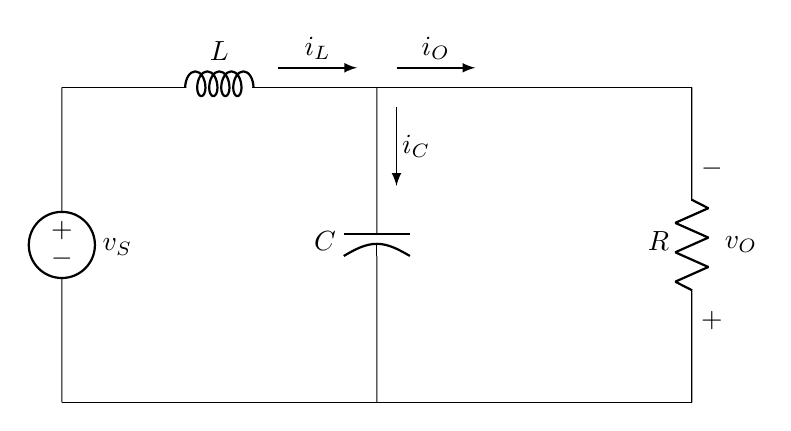
\begin{tikzpicture}[transform shape, american voltages]
	% Paths, nodes and wires:
	\draw (9, 2) to[short] (13, 2);
	\draw (13, 6) to[curved capacitor, l_={$C$}] (13, 2);
	\draw (9, 6) to[cute inductor, l={$L$}] (13, 6);
	\draw (17, 2) to[american resistor, l={$R$}, v=$v_O$, voltage/distance from node=0.7] (17, 6);
	\draw (13, 2) to[short] (17, 2);
	\draw (13, 6) to[short] (17, 6);
	\draw[line width=0.6pt, -latex] (11.75, 6.25) -- (12.75, 6.25);
	\node[shape=rectangle, minimum width=0.465cm, minimum height=0.465cm](N1) at (12.25, 6.5){} node[anchor=center] at (N1.text){$i_L$};
	\draw[line width=0.6pt, -latex] (13.25, 5.75) -- (13.25, 4.75);
	\node[shape=rectangle, rotate=-90, minimum width=0.465cm, minimum height=0.465cm](N2) at (13.5, 5.25){} node[anchor=center] at (N2.text){$i_C$};
	\draw[line width=0.6pt, -latex] (13.25, 6.25) -- (14.25, 6.25);
	\node[shape=rectangle, minimum width=0.465cm, minimum height=0.465cm](N3) at (13.75, 6.5){} node[anchor=center] at (N3.text){$i_O$};
	\draw (9, 6) to[american voltage source, l={$v_S$}] (9, 2);
\end{tikzpicture}

\newpage
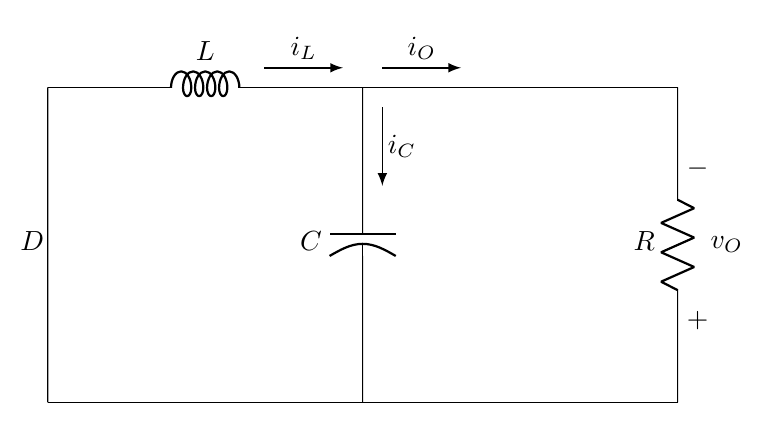
\begin{tikzpicture}[transform shape, american voltages]
	% Paths, nodes and wires:
	\draw (9, 2) to[short] (13, 2);
	\draw (13, 6) to[curved capacitor, l_={$C$}] (13, 2);
	\draw (9, 6) to[cute inductor, l={$L$}] (13, 6);
	\draw (17, 2) to[american resistor, l={$R$}, v=$v_O$, voltage/distance from node=0.7] (17, 6);
	\draw (13, 2) to[short] (17, 2);
	\draw (13, 6) to[short] (17, 6);
	\draw[line width=0.6pt, -latex] (11.75, 6.25) -- (12.75, 6.25);
	\node[shape=rectangle, minimum width=0.465cm, minimum height=0.465cm](N1) at (12.25, 6.5){} node[anchor=center] at (N1.text){$i_L$};
	\draw[line width=0.6pt, -latex] (13.25, 5.75) -- (13.25, 4.75);
	\node[shape=rectangle, rotate=-90, minimum width=0.465cm, minimum height=0.465cm](N2) at (13.5, 5.25){} node[anchor=center] at (N2.text){$i_C$};
	\draw[line width=0.6pt, -latex] (13.25, 6.25) -- (14.25, 6.25);
	\node[shape=rectangle, minimum width=0.465cm, minimum height=0.465cm](N3) at (13.75, 6.5){} node[anchor=center] at (N3.text){$i_O$};
	\draw (9, 6) to[short, l_={$D$}, label distance=-0.3cm] (9, 2);
\end{tikzpicture}

\end{document}